\documentclass[conference]{IEEEtran}
\usepackage{cite}
\usepackage{amsmath,amssymb,amsfonts}
\usepackage{algorithmic}
\usepackage{graphicx}
\usepackage{textcomp}
\usepackage{xcolor}
\def\BibTeX{{\rm B\kern-.05em{\sc i\kern-.025em b}\kern-.08em
    T\kern-.1667em\lower.7ex\hbox{E}\kern-.125emX}}


\begin{document}

\title{CMP9135M | Computer Vision}

\author{\IEEEauthorblockN{1\textsuperscript{st} George Davies}
    \IEEEauthorblockA{
        \textit{School of Computer Science} \\
        \textit{University of Lincoln}\\
        Lincoln, United Kingdom \\
        27421138@students.lincoln.ac.uk
    }
}

\maketitle

\begin{abstract}
\end{abstract}

\begin{IEEEkeywords}
\end{IEEEkeywords}

\section*{Task 1 | Image Processing}

\subsection*{Task 1.a | Automated ball objects segmentation}

\subsection*{Task 1.b | Segmentation evaluation}


\begin{figure}[htbp]
    \centering
    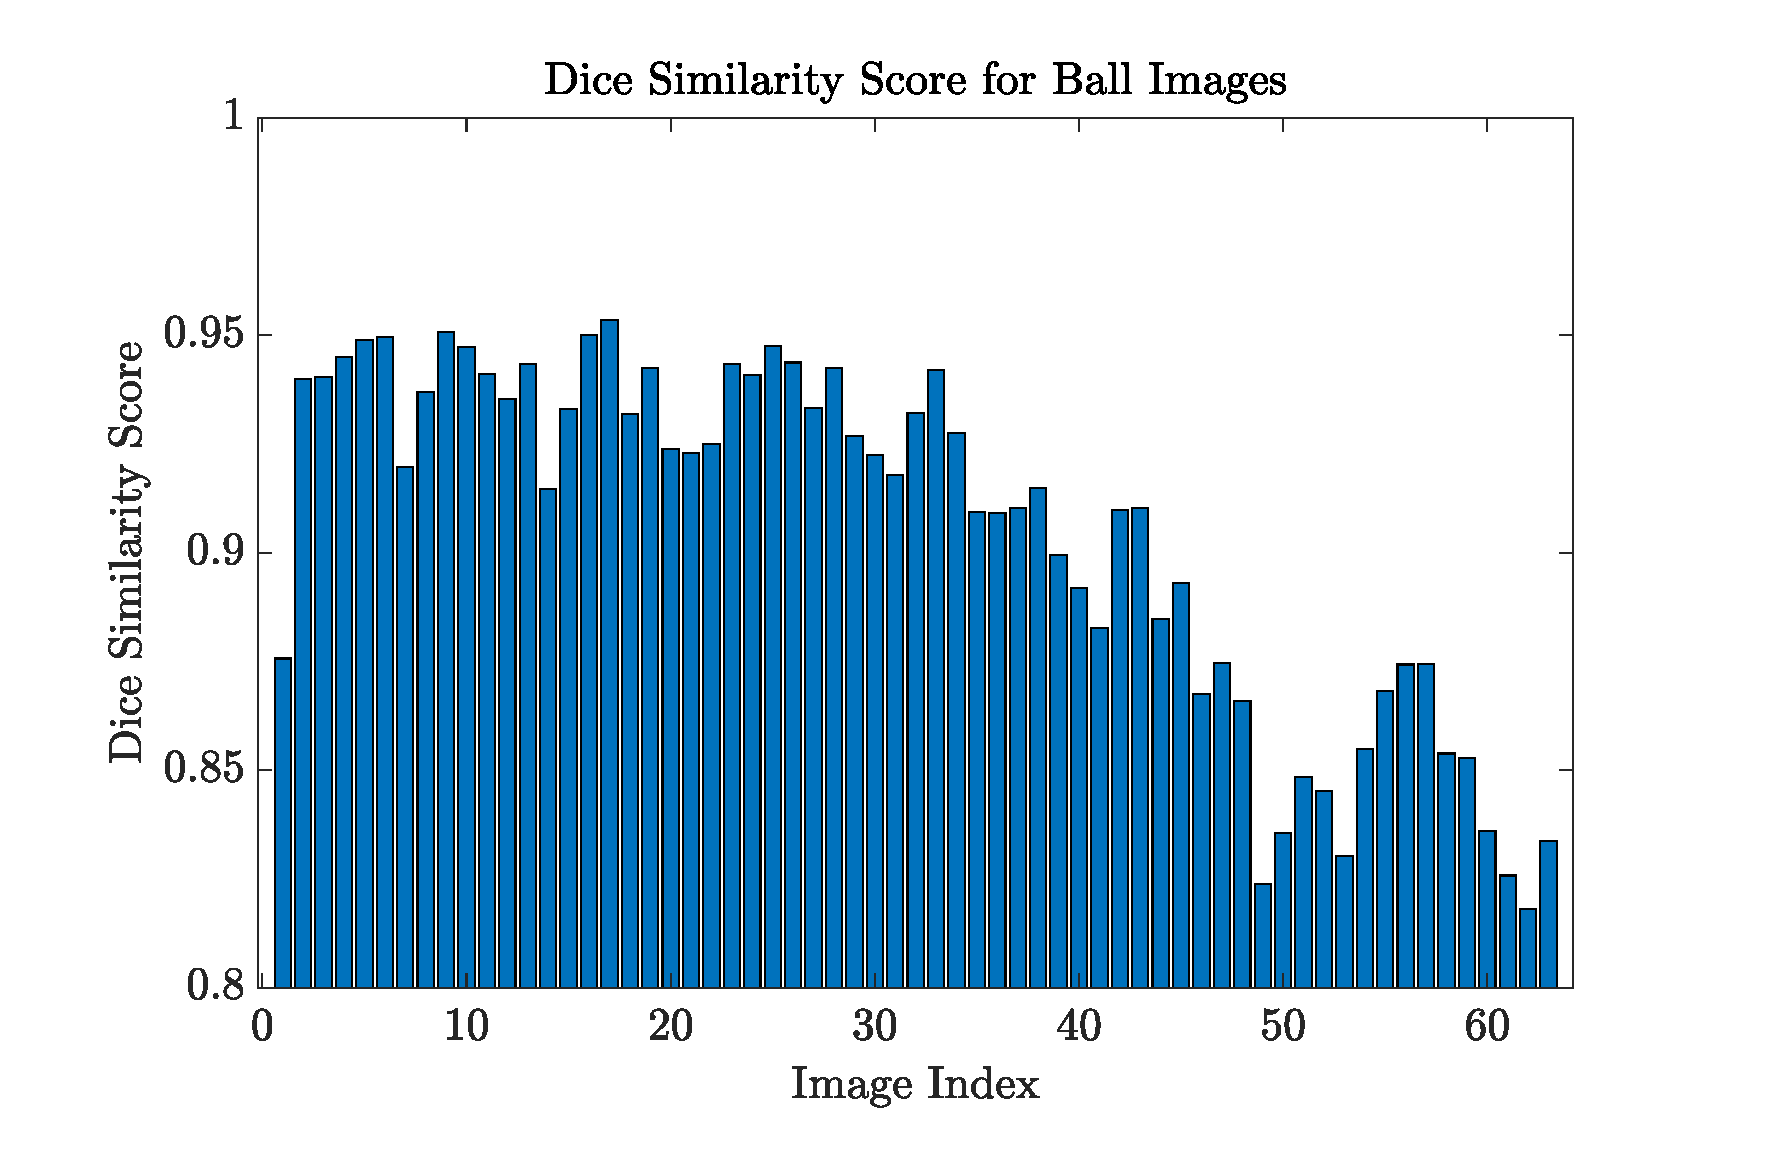
\includegraphics[width=\columnwidth]{figures/DS_bar_graph.pdf}
    \caption{Dice Similarity score for all 63 images\label{apx:best}}
\end{figure}

\section*{Task 2 | Feature Calculation}

\subsection*{Task 2.a | Shape features}

\begin{figure}[htbp]
    \centering
    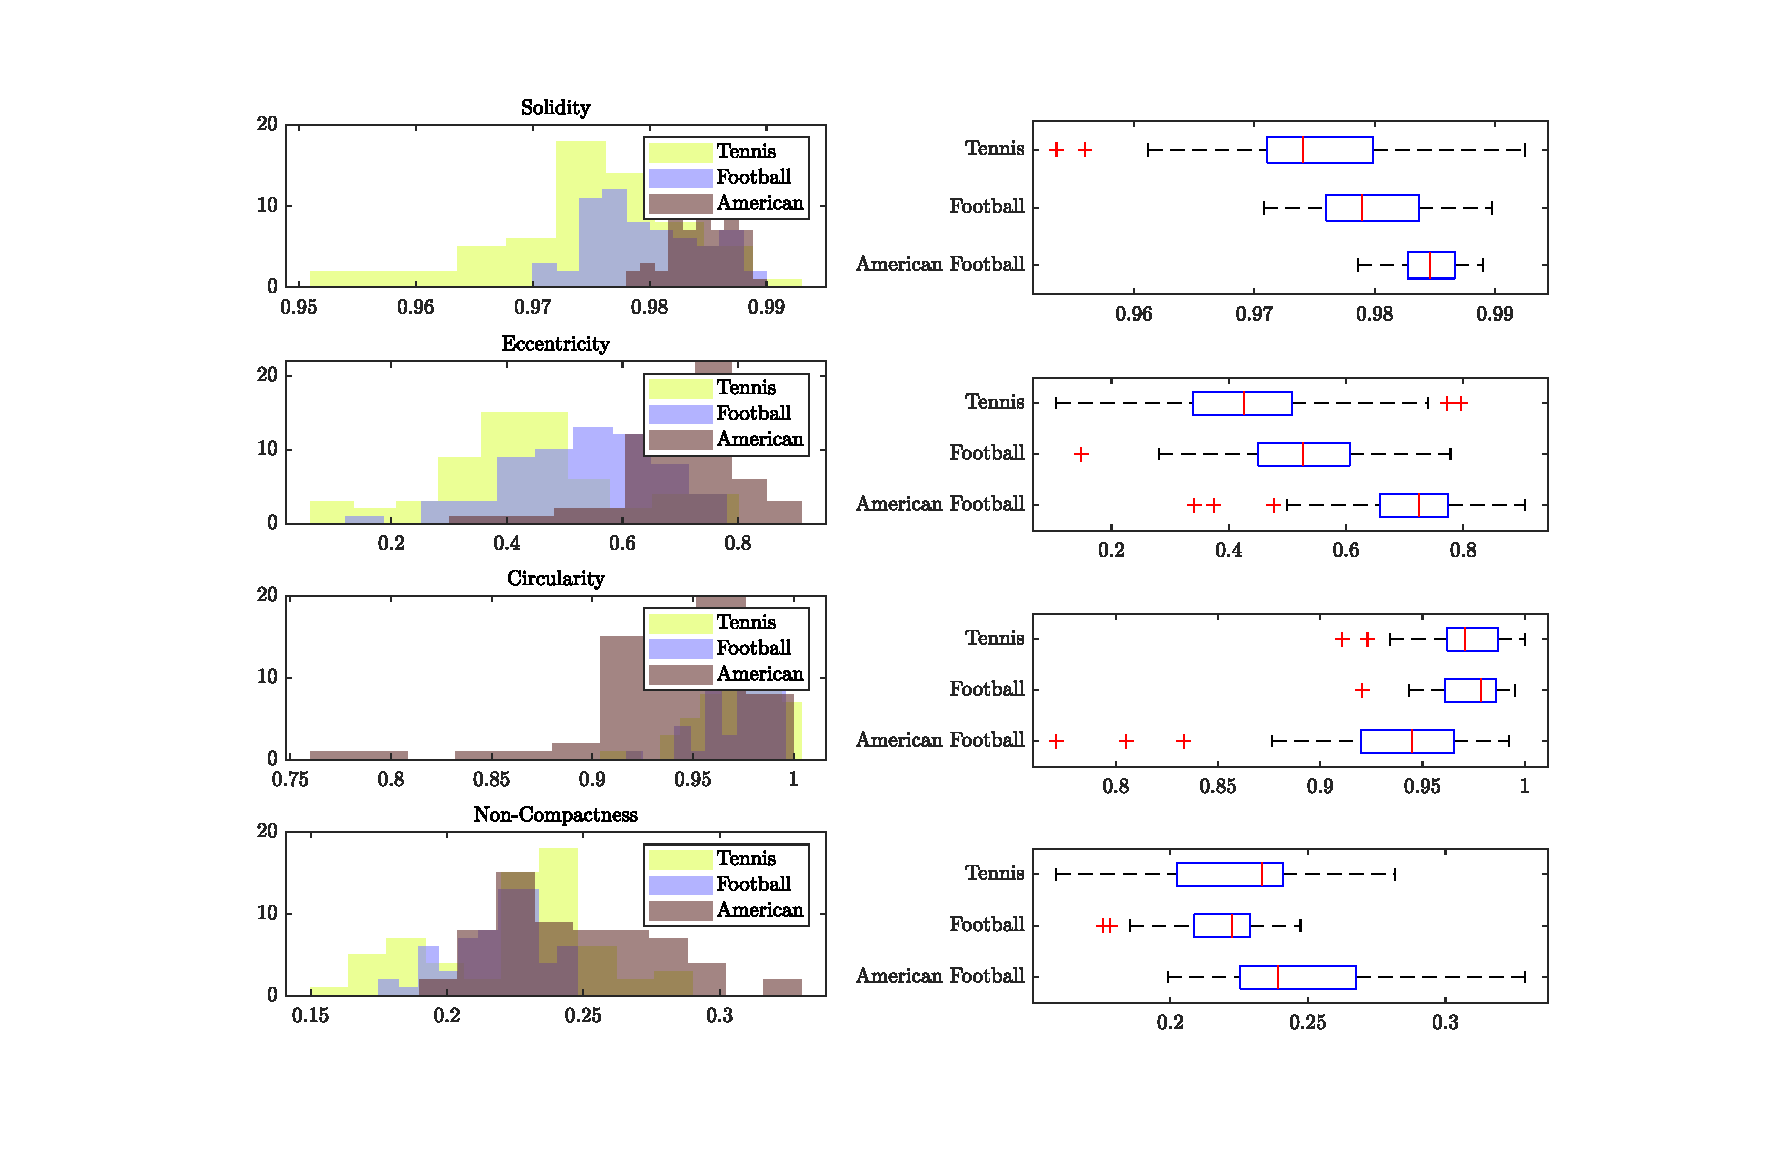
\includegraphics[width=\columnwidth]{figures/shape_feats.pdf}
    \caption{Shape features\label{fig:shape_feats}}
\end{figure}


\subsection*{Task 2.b | Texture features}

\begin{figure}[htbp]
    \centering
    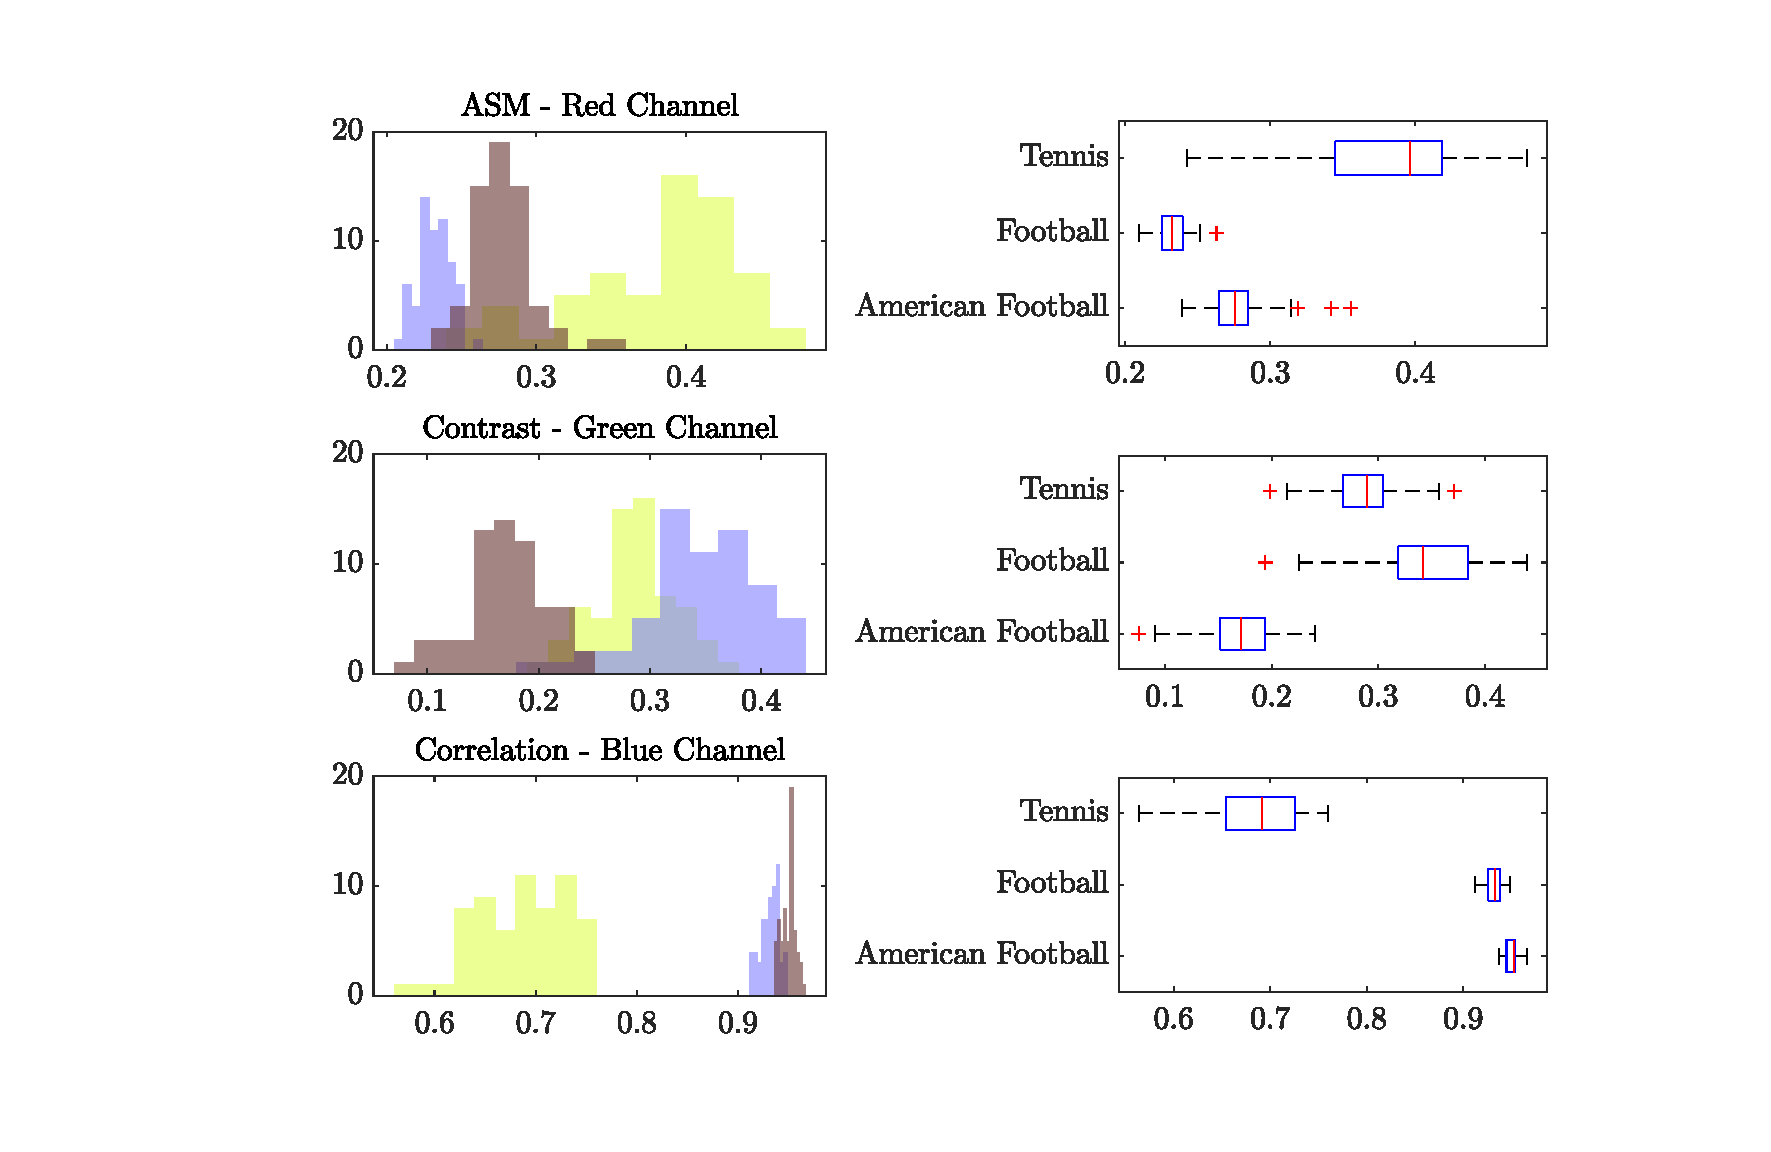
\includegraphics[width=\columnwidth]{figures/averages.pdf}
    \caption{Texture features Averages\label{fig:tex_feats_avgs}}
\end{figure}

\begin{figure}[htbp]
    \centering
    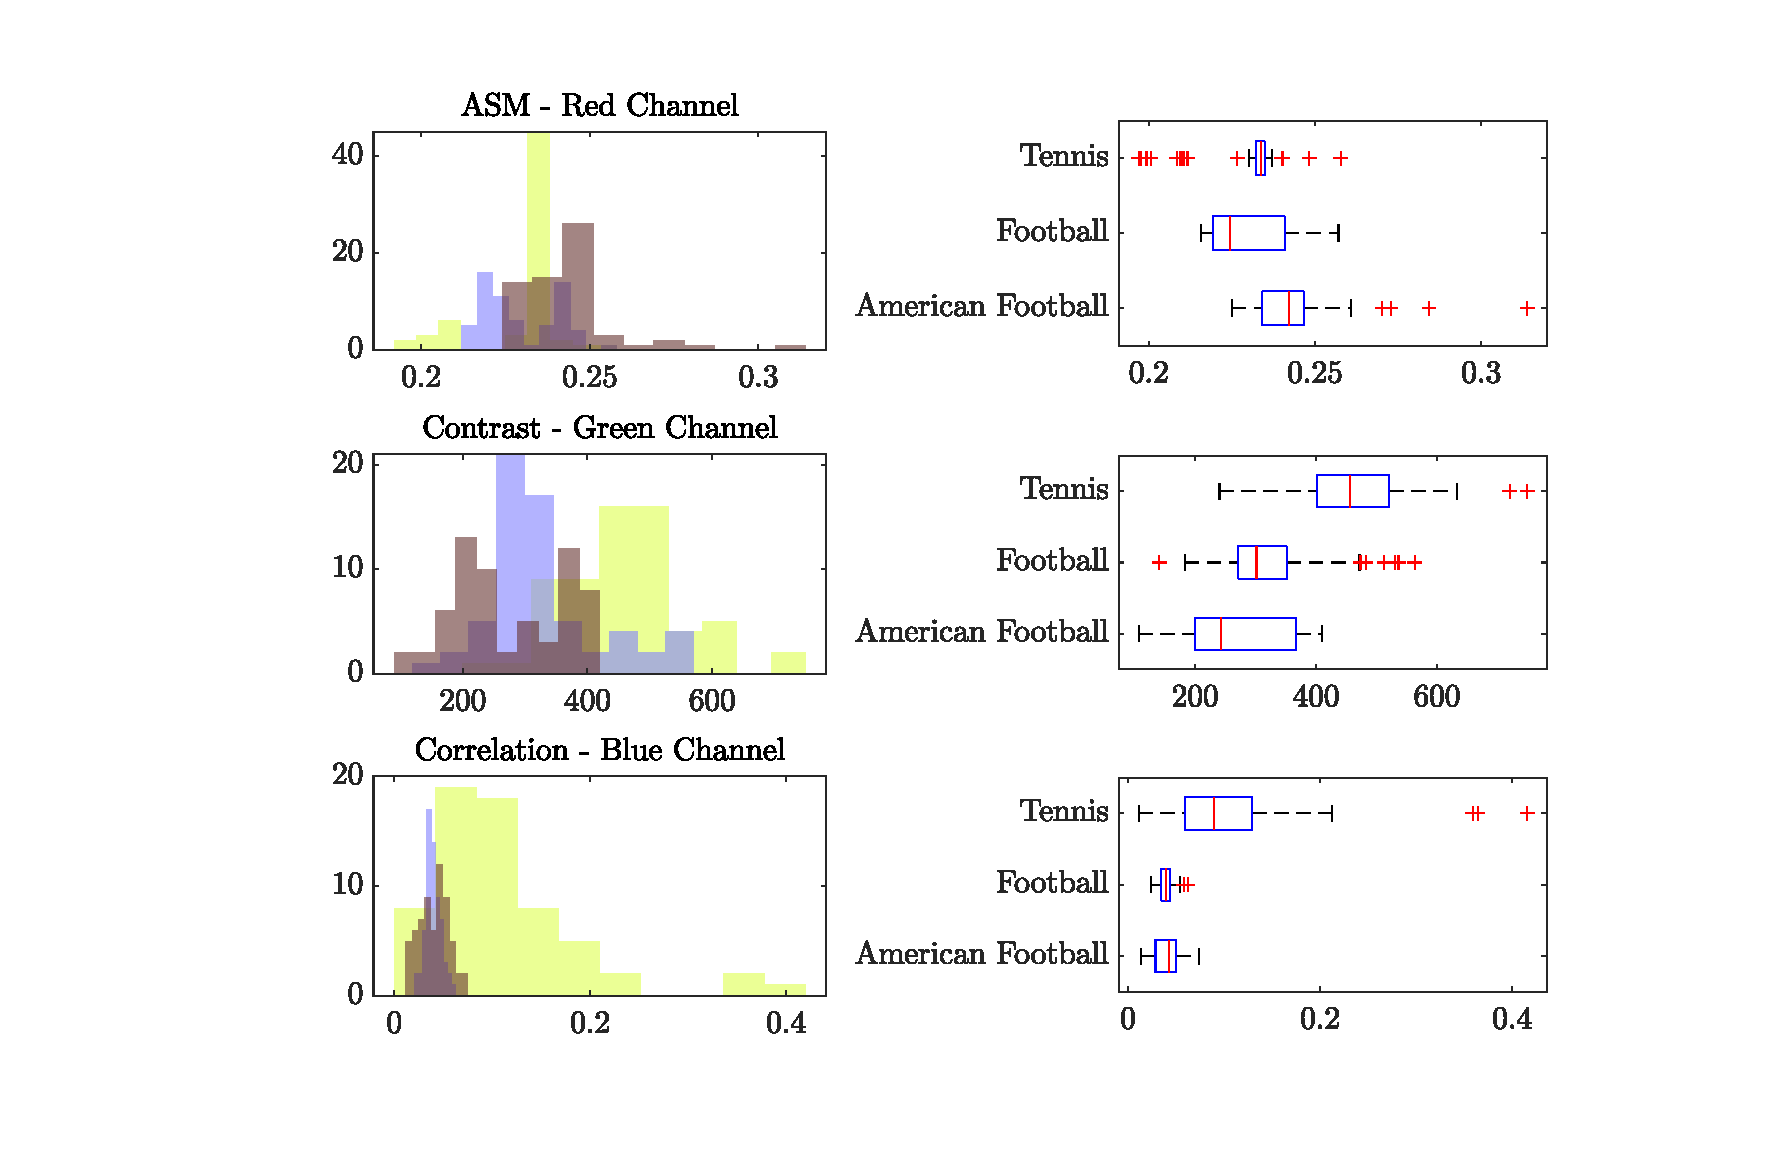
\includegraphics[width=\columnwidth]{figures/ranges.pdf}
    \caption{Texture features Ranges\label{fig:tex_feats_ranges}}
\end{figure}


\subsection*{Task 2.c | Discriminative information}

\section*{Task 3 | Object Tracking}

\subsection*{Task 3.a | Kalman filter tracking}

\subsection*{Task 3.b | Evaluation}


\appendix

\begin{figure}[htbp]
    \centering
    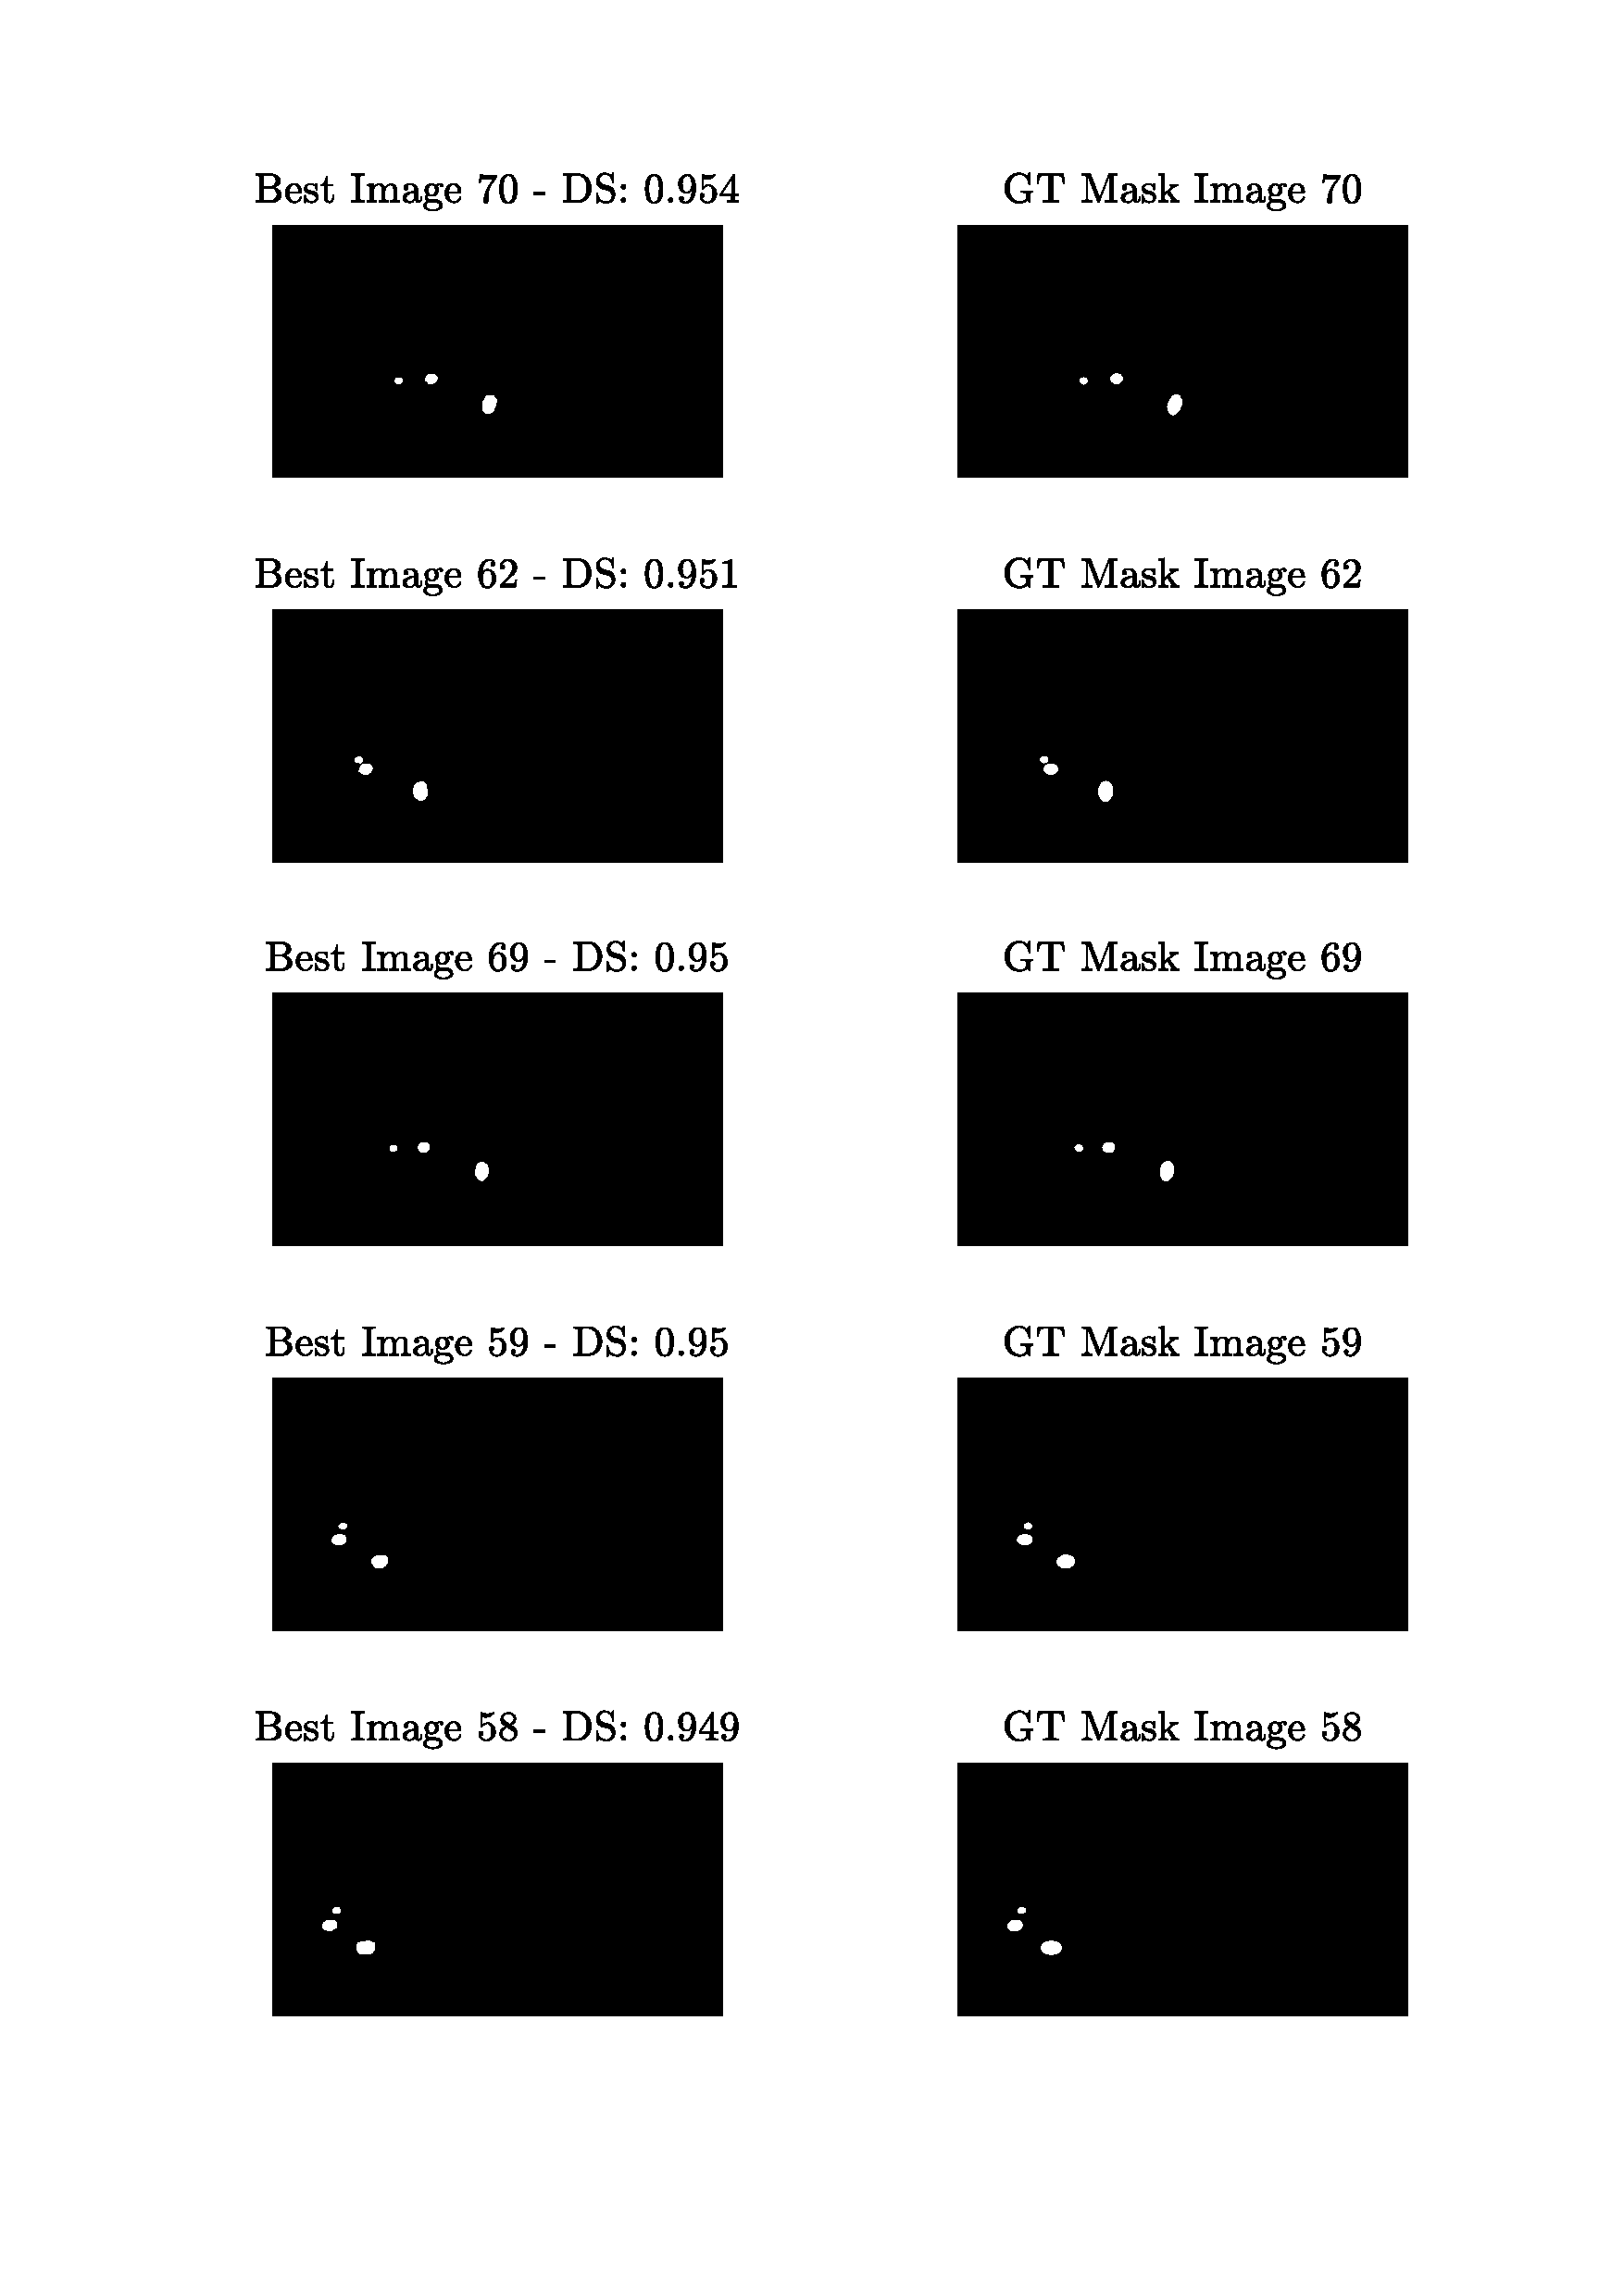
\includegraphics[width=\columnwidth]{figures/best.pdf}
    \caption{Best 5 segmented ball images compared to the ground truth\label{apx:best}}
\end{figure}
\begin{figure}[htbp]
    \centering
    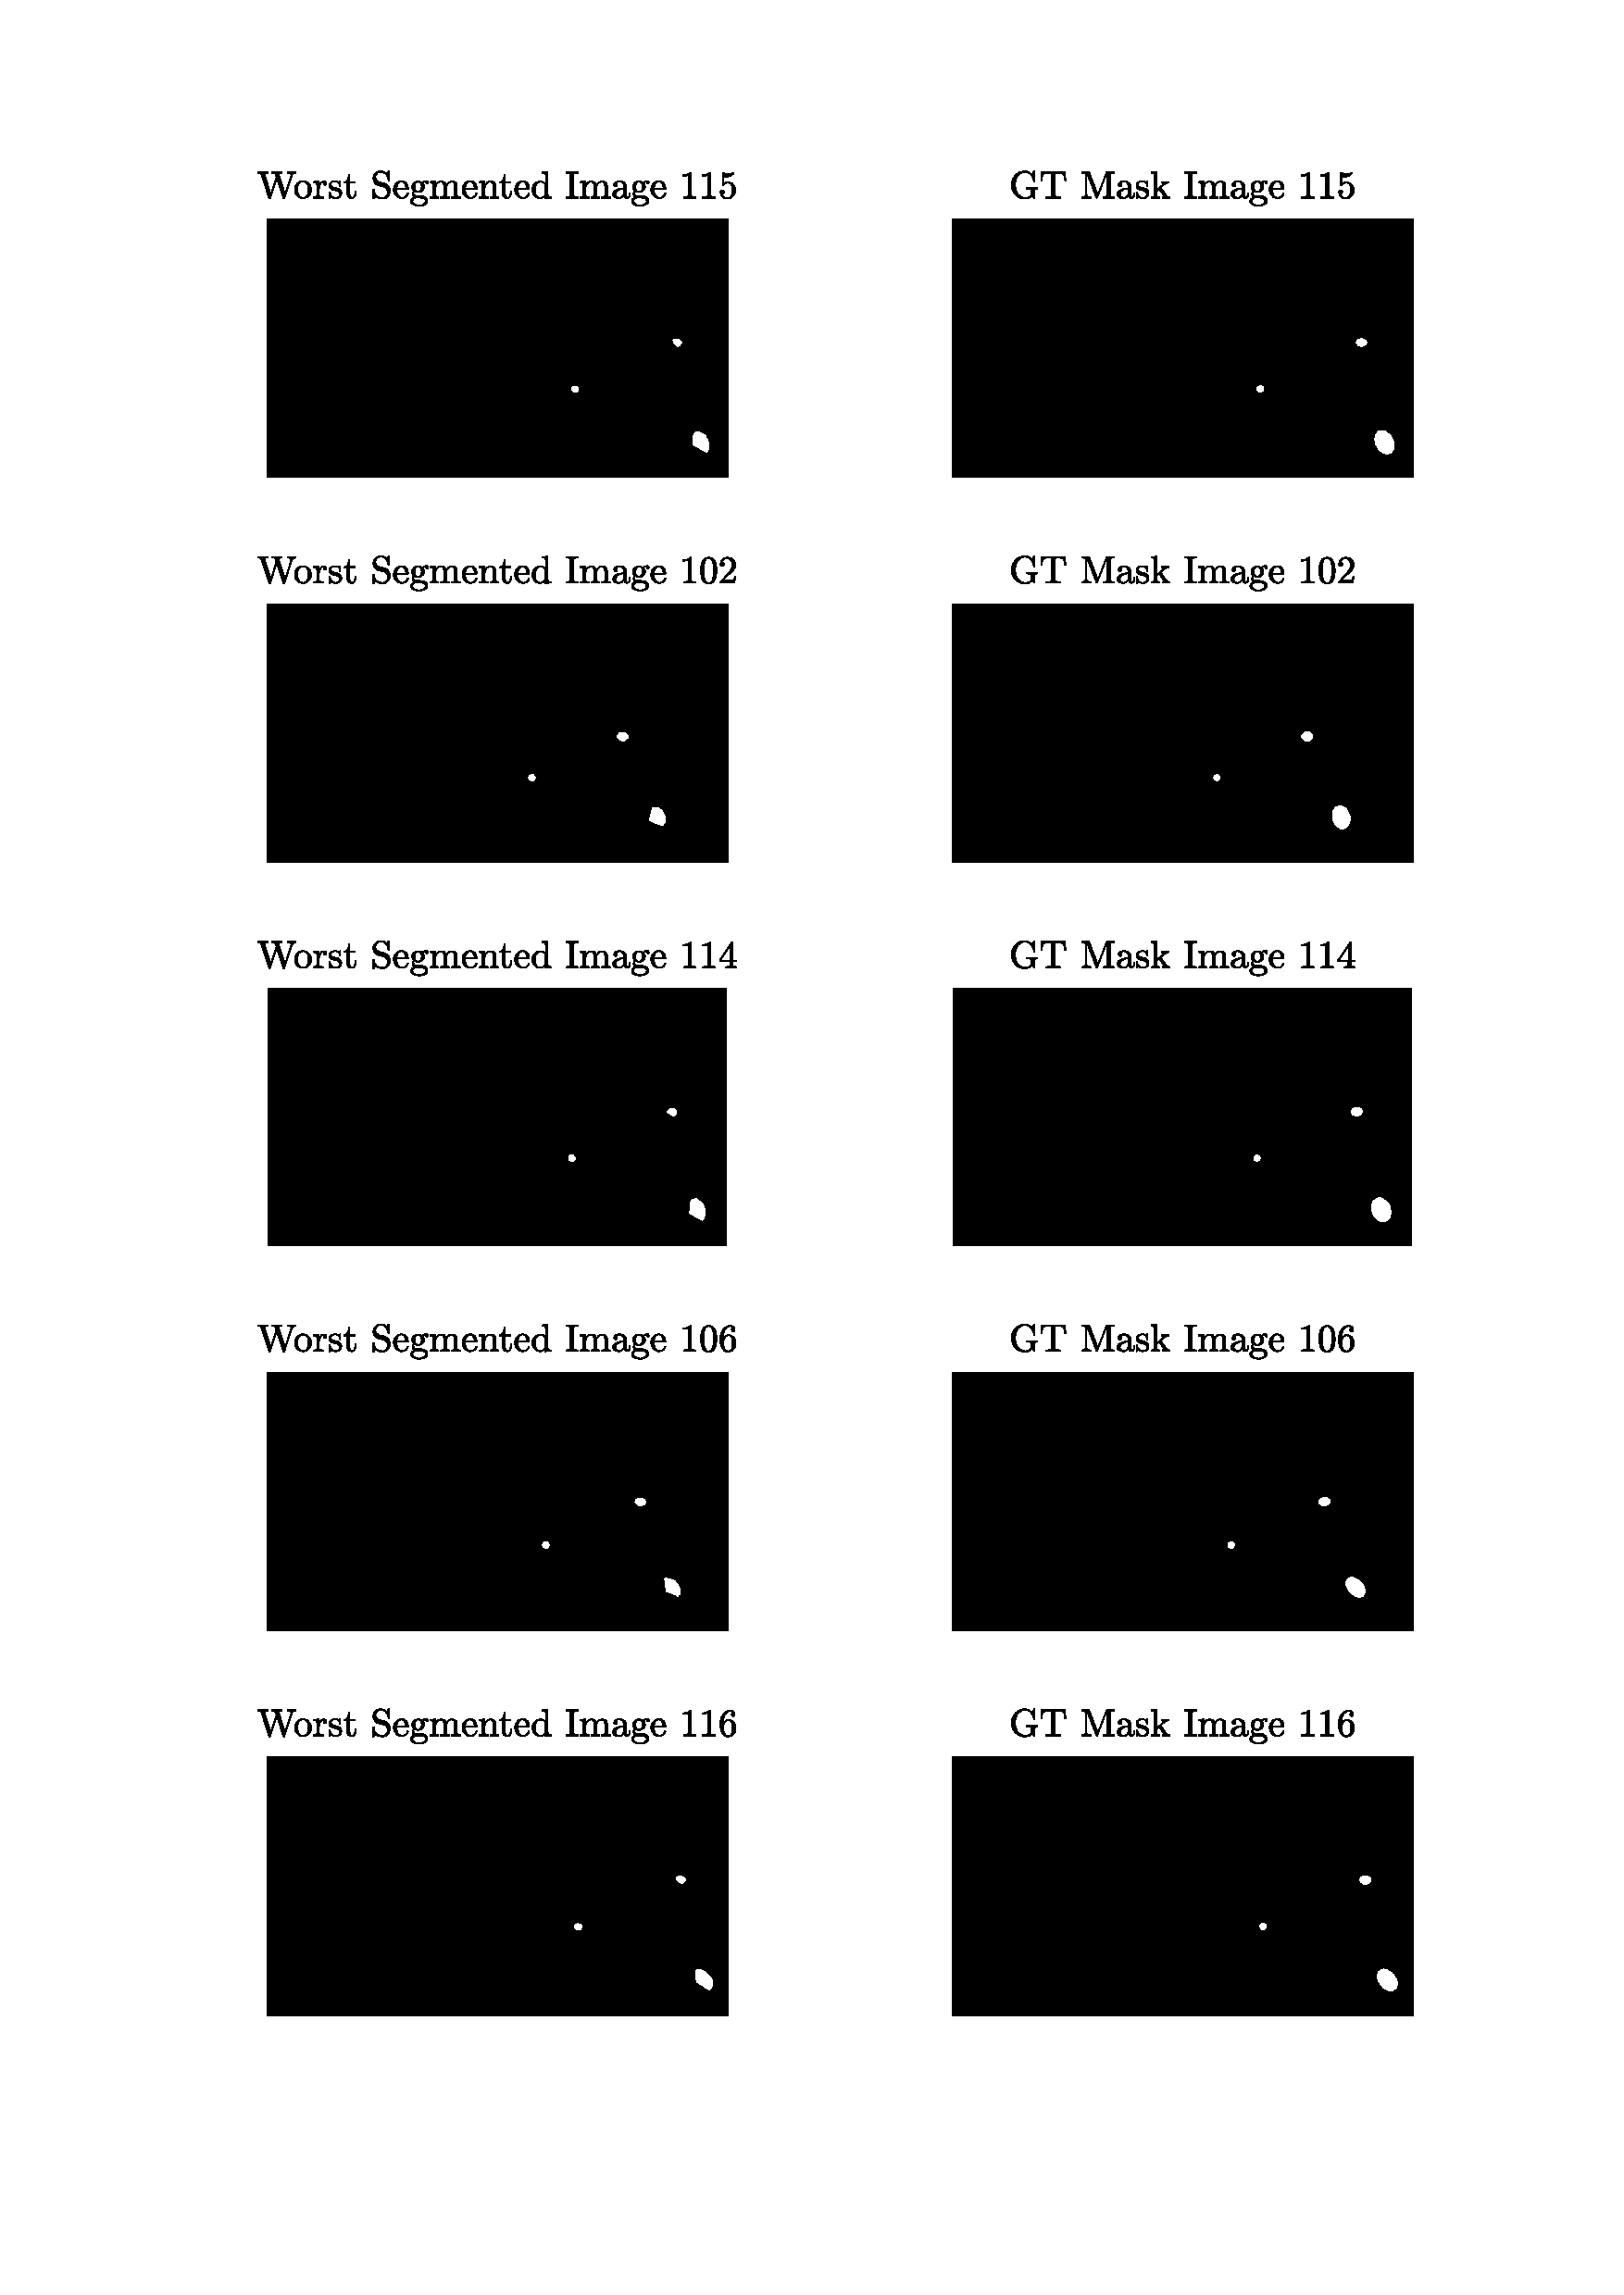
\includegraphics[width=\columnwidth]{figures/worst.pdf}
    \caption{Worst 5 segmented ball images compared to the ground trut\label{apx:worst}}
\end{figure}


\end{document}
